\chapter{Functions}

\begin{wrapfigure}{l}{4cm}
  \begin{center}
    \vskip -0.5cm
    \qrset{link, height=3cm}
    \qrcode{https://youtu.be/VHJeUrCedTU}
    \vskip 0.25cm
    \href{https://youtu.be/VHJeUrCedTU}{youtu.be/VHJeUrCedTU}
    {\footnotesize Functions and Quantifiers}
  \end{center}
  \vskip -0.5cm
\end{wrapfigure}

Another important type of objects in mathematics are functions. Function $f$
from a set $X$ to a set $Y$ (we write it as $f : X \to Y$) is a unique
assignment of elements of $Y$ to the elements of $X$. In other words, for each
element $x \in X$ there is one assigned element $f(x) \in Y$. We call such an
element the \textit{value} of $f$ at $x$, we also say that $f(x)$ is an
\textit{image} of $x$.

Unfortunately, the definition is not formal. In the rest of the chapter we are
going to give a more formal definition.

\section{Quantifiers.}
The first ingredient is called quantifiers. Very often we use phrases like ``all
the people in the class have smartphones.'' However, we still do not know how to
write it using symbols.

\paragraph{The Universal Quantifier.}
In order to say ``all'' or ``every'' we use the symbol $\forall$: if
$P(a)$ is a predicate about $a \in A$, then $\forall a \in A\ P(a)$ is a
statement saying that all the elements of $A$ satisfy the predicate $P$. In
other words it is the same as the statement
$\set[P(a)]{a \in A} = A$. For example, $\forall x \in \R\ x \cdot 0 = 0$ says
that product of every real number and zero is equal to zero.

\paragraph{The Existential Quantifier.}
The second quantifier means ``there is'' and denoted by the symbol $\exists$:
if $P(a)$ is a predicate about an element of $A$, then $\exists a \in A\ P(a)$
says that there is an element of $A$ satisfying the predicate $P$ i.e.
$\set[P(a)]{a \in A} \neq \emptyset$. For example,
$\exists x \in \R\ x^2 - 1 = 0$ states that there is a real solution of the
equation $x^2 - 1 = 0$.

\begin{warning}
  Note that the word ``any'' sometimes indicates a universal statement and
  sometimes an existential statement.

  Standard meaning of ``any'' is ``ever'' like in the statement ``$a^2 \ge 0$
  for any real number'', therefore this statement can be rewritten as
  $\forall a \in \R \ a^2 \ge 0$. Nonetheless, in the negative and interrogative
  statements ``any'' is used to mean ``some''. For example, ``There is not any
  real number $a$ such that $a^2 < 0$'' is asserting that the statement
  $\exists a \in \R \ a^2 < 0$ is false. And ``Is there any real number $a$ such
  that $a^2 = 1$?'' is asking whether the existential statement
  $\exists a \in \R \ a^2 = 1$ is true.

  Real care is required with questions involving ``any'': ``Is there any
  integer $a$ such that $a \ge 1$?'' clearly is asking whether $\exists a \in
  \R \ a^2 \ge 1$ is true; however, ``Is $a \ge 1$ for any integer $a$'' is less
  clear and might be taken to asking about the same question as the first
  question, $\exists a \in \Z \ a \ge 1$ (which is true) but might also be
  taken to be asking about $\forall a \in \Z \ a \ge 1$ (which is false).
\end{warning}

\subsection{Proving Statements Involving Quantifiers}
Most of the statements in mathematics involve quantifiers. This is one of the
factors distinguishing advanced from elementary mathematics. In this section we
give an overview of the main methods of proof. Though the whole book is about
proving such results.

\paragraph{Proving statements of the form $\forall a \in A \ P(a)$.}
Such statements can be rewritten in the form $a \in A \implies P(a)$. For
example, we proved earlier that $a^2 \ge 0$ for all real numbers $a$ using this
approach.

\paragraph{Proving statements of the form $\exists a \in A \ P(a)$.}
The easiest way to prove such a statement is by simply exhibiting an element $a$
of $A$ such that $P(a)$ is true. This method is called \textit{proof by
example}.

Let us prove the statement $\exists x \in \N \ x^2 = 4$ using this method.
Observe that $2 \in N$ and $2^2 = 4$ so $x = 2$ provides an example proving
this statement. There are, however, less direct methods such as use of the
counting arguments.

\paragraph{Proving statements involving both quantifiers.}
To illustrate problems of this type let us prove that for any integer $n$, if
$n$ is even, then $n^2$ is also even.

This statement is a universal statement $\forall n \in \Z \ (n \text{ is even}
\implies n^2 \text{ is even})$. However, the hypothesis that $n$ is even is an
existential statement $\exists q \in \Z \ n = 2q$. So we begin the proof as
follows:
\begin{center}
  Suppose that $n$ is an even integer. Then $n = 2q$ for some integer $q$.
\end{center}
The conclusion we wish to prove is that $n^2$ is even, which may be written as
$\exists q \in \Z \ n^2 = 2q$. Note that $q$ here is a dummy variable used to
express the statement $n^2$ is a doubled integer. We may replace it by any
other letter not already in use, for example $\exists p \in \Z \ n^2 = 2p$.
Hence, if we present $p$ such that $n^2 = 2p$ we finish the proof. As a result,
we can complete the proof as follows.
\begin{center}
  Therefore, $n^2 = (2q)^2 = 4q^2$ and so, since $2q^2$ is an integer $n^2$ is
  even.
\end{center}

\subsection{Disproving Statements Involving Quantifiers}
Disproving something seems a bit off from the first glance, but to some extent
it is the same as proving the negation.

\paragraph{Disproving statements of the form $\forall a \in A \ P(a)$.}
We may note that the negation of such a statement is the statement $\exists a
\in A \ \lnot P(a)$. So we can disprove it by giving a single example for which
it is false. This is called \textit{Disproof by counterexample} to $P(a)$.

For example, we may disprove the statement $\forall x \in \R \ x^2 > 2$ by
giving a counterexample $x = 1$ since $1^2 = 1 < 2$.

\paragraph{Disproving statements of the form $\exists a \in A \ P(a)$.}
The negation of this statement is the statement $\forall a \in A \ \lnot P(a)$.
Which gives one way of disproving the statement.

Let us prove that does not exist a real number $x$ such that $x^2 = -1$. We
know that, for all $x \in \R$, we have the inequality $x^2 \ge 0$ and so $x^2
\neq -1$. Hence, there does not exist $x \in \R$ such that $x^2 = -1$.

\section{Cartesian product}
Another ingredient is the notion of Cartesian product. If $X$ and $Y$ are two
sets, then $X \times Y = \set[x \in X \text{ and } y \in Y]{(x, y)}$. When $X =
Y$ we denote $X \times X = X^2$.

Consider the following example. If $X = \set{a, b, c}$ and $Y = \set{a, b}$,
then $$X \times Y = \set{(a, a), (a, b), (b, a), (b, b), (c, a), (c, b)}.$$
Additionally, $\R^2 = \R \times \R$ is the familiar $2$-dimensional Euclidean
plane.

\begin{exercise}
  Find the set $\set{a, b} \times \set{a, b} \setminus
  \set[x \in \set{a, b}]{(x, x)}$
\end{exercise}

\begin{theorem}
\label{theorem:cartesian-product-distributivity}
  For all sets $A$, $B$, $C$, and $D$ the following hold:
  \begin{itemize}
    \item $A \times (B \cup C) = (A \times B) \cup (A \times C)$;
    \item $A \times (B \cap C) = (A \times B) \cap (A \times C)$;
    \item $(A \times B) \cup (C \times D) \subseteq
      (A \cup B) \times (C \cup D)$;
    \item $(A \times B) \cap (C \times D) =
      (A \cap B) \times (C \cap D)$.
  \end{itemize}
\end{theorem}
\begin{proof}
  It is easy to prove this statement by the definitions. Let us prove only the
  second equality, the rest is
  Exercise~\ref{exercise:cartesian-product-distributivity}.

  Note that $(x, y) \in A \times (B \cap C)$ iff $x \in A$ and
  $y \in (B \cap C)$.
  Hence, $(x, y) \in A \times (B \cap C)$ iff $x \in A$, $y \in B$, and
  $y \in C$. Thus $(x, y) \in A \times (B \cap C)$ iff
  $(x, y) \in (A \times B)$ and $(x, y) \in (A \times C)$. As a result,
  $(x, y) \in A \times (B \cap C)$ iff
  $(x, y) \in (A \times B) \cap (A \times C)$ as required.
\end{proof}


\begin{exercise}
\label{exercise:cartesian-product-distributivity}
  Prove the rest of the equalities in
  Theorem~\ref{theorem:cartesian-product-distributivity}.
\end{exercise}


\section{Graphs of Functions}
\label{section:graph}
Now we have all the components to define a function. Mathematicians think about
the functions in the way we defined them at the beginning of the chapter,
however formally in order to define a function $f : X \to Y$ one need to define
a set $D \subseteq X \times Y$ (such a set is called the \textit{graph of the
function} $f$) such that
\begin{itemize}
  \item $\forall x \in X~\exists y \in Y\ (x, y) \in D$ and
  \item $\forall x \in X, y_1, y_2 \in Y\
    ((x, y_1) \in D \land (x, y_2) \implies y_1 = y_2)$.
\end{itemize}
We say that $y \in Y$ is the value $f(x)$ of the function described by $D$ at
$x \in X$ iff $(x, y) \in D$.

The simplest way to think about the functions is in the terms of tables.
Let us use this idea to list all the functions $\set{a, b, c}$ to $\set{d, e}$.
\begin{center}
  \begin{tabular}{c | c | c | c | c | c | c | c | c}
    $x$ & $f_1(x)$ & $f_2(x)$ & $f_3(x)$ & $f_4(x)$ & $f_5(x)$ & $f_6(x)$ &
    $f_7(x)$ & $f_8(x)$ \\
    \hline
    a & d & d & d & d & e & e & e & e \\
    b & d & d & e & e & d & d & e & e \\
    c & d & e & d & e & d & e & d & e
  \end{tabular}
\end{center}

\begin{exercise}
  List all the functions from $\set{a, b}$ to $\set{a, b}$.
\end{exercise}

However, listing all the values of a function is only possible when the domain
of the function is finite. Thus the most common way to describe a function is
using a formula which provides a way to find the value of a function. When the
function is defined as a formula it is important to be clear which sets are the
domain and the codomain of the function.

Let $\R_+ = \set[x \ge 0]{x \in \R}$. Consider the following functions.
\begin{itemize}
  \item $f_1 : \R \to \R$ such that $f_1(x) = x^2$;
  \item $f_1 : \R_+ \to \R$ such that $f_1(x) = x^2$;
  \item $f_1 : \R \to \R_+$ such that $f_1(x) = x^2$;
  \item $f_1 : \R_+ \to \R_+$ such that $f_1(x) = x^2$;
\end{itemize}
Nonetheless that all these functions are defined using the same formula $x^2$,
we will see in the next chapters that these four functions have different
properties.

\begin{exercise}
  Find the graph of the function $f : \Z \to \Z$ such that $f(x) = 3x$.
\end{exercise}

Note that when you define the function you need to define it such that the
definition makes sense for all the elements of the domain. For example, the
formula $g(x) = \frac{x^2 - 3x + 2}{x - 1}$ does not define a function from
$\R$ to $\R$ since it is not defined for $x = 1$. It is typical to define a
function from real numbers to real numbers by a formula and the convention is
that the domain is the set of all numbers for which the formula makes sense
(unless the domain is specified explicitly).
Using this convention the formula $g$ defines a function from $\R \setminus
\set{1}$ to $\R$.

If we really need a function from $\R$ there are two possible approaches for
extending $g$.

\paragraph{Rewriting the formula.}
We can rewrite the formula such that it makes sense for all the real numbers.
Note that for all $x \in \R \setminus \set{1}$,
\[
  \frac{x^2 - 3x + 2}{x - 1} = \frac{(x - 2)(x - 1)}{x - 1} = x - 2.
\]
Then $g_1(x) = x - 2$ defines a function on $\R$ extending the function $g$.

\paragraph{Explicit definition.} Alternatively we can explicitly specify the
value of $g$ at $1$. So
\[
  g_2(x) =
  \begin{cases}
    \frac{x^2 - 3x + 2}{x - 1} & \text{if } x \neq 1 \\
    -1 & \text{if } x = 1
  \end{cases}
\]
defines a function from $\R$ to $\R$. Note that we can specify the values at
individual points any way we want.

Similarly to sets we may define the equality between functions. We say that two
functions $f, g : X \to Y$ are equal ($f = g$) iff $f(x) = g(x)$ for all
$x \in X$ i.e. their graphs are equal. Note that two functions are equal only
if they have the same domains and codomains. For example, $g_1$ and $g_2$ we
just defined are equal to each other none the less that we defined them in two
different ways.

We defined $g_1$ and $g_2$ to extend $g$ to a bigger domain, similarly we can
make a domain smaller.
\begin{definition}
  Let $f : X \to Y$ and $A \subseteq X$. Then $f|_{A} : A \to Y$ is a function
  such that $\forall x \in A\ f|_{A}(x) = f(x)$.
\end{definition}

\section{Composition of Functions}
\begin{center}
    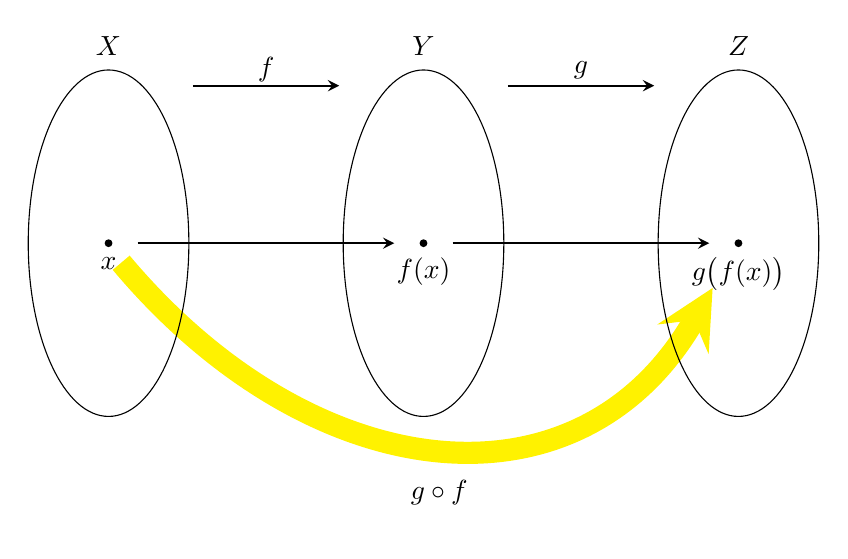
\begin{tikzpicture}[
    >=stealth,
    bullet/.style={
        fill=black,
        circle,
        minimum width=1pt,
        inner sep=1pt
    },
    projection/.style={
        ->,
        thick,
        shorten <=2pt,
        shorten >=2pt
    },
    every fit/.style={
        ellipse,
        draw,
        inner sep=0pt
    }
    ]
    \node at (2,4.7) {$f$};
    \draw[projection] (1,4.5) -- (3,4.5);
    \node at (0,5) {$X$};
    \node[bullet,label=below:$x$] (START)   at (0,2.5){};
    \node at (4,5) {$Y$};
    \node[bullet,label=below:$f(x)$] at (4,2.5){};
    \node at (6,4.7) {$g$};
    \draw[projection] (5,4.5) -- (7,4.5);
    \node at (8,5) {$Z$};
    \node[bullet,label=below:$g\big(f(x)\big)$] (END) at (8,2.5){};

    \draw [line width=8pt, yellow, shorten <=0.25cm,, shorten >=0.6cm, ->] (START.south) to[out=-50, in=-120, distance=4cm, ] node[black, midway, below, align = center, yshift = -0.25cm] {$g \circ f$} (END);

    \draw (0,2.5) ellipse (1.02cm and 2.2cm);
    \draw (4,2.5) ellipse (1.02cm and 2.2cm);
    \draw (8,2.5) ellipse (1.02cm and 2.2cm);

    \draw[projection] (0.3,2.5) -- (3.7,2.5);
    \draw[projection] (4.3,2.5) -- (7.7,2.5);
    \end{tikzpicture}
    \newline
\end{center}

Suppose $f : X \ to Y$ and $g : Y \to Z$ be some function. Then, given an
element $x \in X$, the function $f$ assigns $y = f(x) \in Y$, and the function
$g$ assigns $z = g(y) = g(f(x)) \in Z$. Thus using $f$ and $g$ an element of
$Z$ can be assigned to $x$. This operation defines a function from $X$ to $Z$
and the result of this operation is called the \textit{composition} of $f$ and
$g$.

\begin{definition}
  If $f : X \to Y$ and $g : Y \to Z$, then $h = g \circ f$ is a
  function from $X$ to $Z$ such that $\forall x \in X\ g(f(x)) = h(x)$.
\end{definition}.

Let us consider an example. Let $f : \R \to \R$ such that $f(x) = x + 1$ and
$g : \R \to \R$ such that $g(x) = x^2$. Then $(g \circ f) : \R \to \R$ and
$(g \circ f)(x) = (x + 1)^2$ for all $x \in \R$. Note that the order of $f$ and
$g$ is important since $(f \circ g)(x) = x^2 + 1$. Thus composition is not
\textit{commutative}.

There are two special type functions.
\begin{itemize}
  \item Let $A \subseteq X$, then $i : A \to X$ such that $i(a) = a$ for all
    $a \in A$ is called the \textit{inclusion} function of $A$ into $X$. Observe
    that $(f \circ i) : A \to X$ and $(f \circ i) = f|_A$
    for any function $f : X \to Y$.
  \item Another important function is called the \textit{identity} function.
    Let $X$ be some set. Then $I_X : X \to X$ is an identity function iff
    $I_X(x) = x$.
\end{itemize}

\begin{theorem}
  Let $f : X \to Y$, $g : Y \to Z$, and $h : Z \to W$. Then
  \begin{itemize}
    \item $f \circ (g \circ h) = (f \circ g) \circ h$.
    \item $f \circ I_X = f = I_Y \circ f$.
  \end{itemize}
\end{theorem}
\begin{proof}
  These results can be proven simply by evaluating the functions. For example,
  both functions in the first equality assign $h(g(f(x)))$ for any $x \in X$
  and so functions are equal.
\end{proof}
Notice that this theorem states that we may write $f \circ g \circ h$ without
ambiguity.

\section{The Image of a Function}
Given a function $f : X \to Y$, it is not necessary that every element of $Y$
is an image of some $x \in X$. For example, the function $\R \to \R$ defined by
the formula $x^2$ does not have $-1$ as a value.

Thus we may give the following definition.
\begin{definition}
  The image of the function $f$ is defined as follows
  $$\Im f = \set[\exists x \in X\ f(x) = y]{y \in Y}
  = \set[x \in X]{f(x)}$$ (in other
  words it is the projection of the graph $D$ of $f$ on the second coordinate:
  $\Im f = \set[(x, y) \in D]{y}$).
\end{definition}

\section*{End of The Chapter Exercises}
\begin{exercises}
  \exerciseitem Find an image of the function $f : \Z \to \Z$ such that
    $f(x) = 3x$.
  \exerciseitem Determine the following sets:
    \begin{itemize}
      \item $\set[\exists n \in N \ m \le n]{m \in \N}$;
      \item $\set[\forall n \in N \ m \le n]{m \in \N}$;
      \item $\set[\exists m \in N \ m \le n]{n \in \N}$;
      \item $\set[\exists m \in N \ m \le n]{n \in \N}$.
    \end{itemize}
  \exerciseitem Prove or disprove the following statements.
    \begin{itemize}
      \item $\forall m, n \in \N \ m \le n$.
      \item $\exists m, n \in \N \ m \le n$.
      \item $\exists m \in \N \forall n \in \N \ m \le n$.
      \item $\forall m \in \N \exists n \in \N \ m \le n$.
      \item $\exists n \in \N \forall m \in \N \ m \le n$.
      \item $\forall n \in \N \exists m \in \N \ m \le n$.
    \end{itemize}
\end{exercises}
